\documentclass[10pt]{article}
\usepackage[english]{babel}									
\usepackage[utf8]{inputenc}									
\usepackage[T1]{fontenc}									\usepackage{url}	

\usepackage{amsmath,amsfonts,amssymb,amsthm,cancel,siunitx,
calculator,calc,mathtools,empheq,latexsym}
\usepackage{subfig,epsfig,tikz,float}		           
\usepackage{booktabs,multicol,multirow,tabularx,array}        
\usepackage[numbers, super]{natbib}
\usepackage{graphicx}
\usepackage{capt-of}
\setlength{\parindent}{0pt}
\setlength{\parskip}{10pt}
\textwidth 13.5cm
\textheight 19.5cm
\columnsep .5cm
\usepackage{geometry}
\geometry{a4paper, portrait, margin=1in}
\title{\renewcommand{\baselinestretch}{1.17}\normalsize\bf%
\uppercase{Technical Analysis Between Weather, Total Load, and Price in Spain}
}
\setcitestyle{square}

\begin{document}
\date{}
\maketitle

\vspace{-0.5cm}

\begin{center}
{\footnotesize 
ECS 171 Machine Learning - Group 25
}
\end{center}

\begin{center}
{\footnotesize 
Jacqueline Mitchell, Ameya Naik, Joshua Peterson, Hashim Chaudhry, Claire Wong, Shreyas Vankayalapati, Bhargava Sharma
}
\end{center}
\bigskip
\noindent
%{\small{\bf ABSTRACT.}
%Abstract should concisely
%summarize the key findings of the paper. It should consist 
%of a single paragraph containing no more than 150 words. 
%The Abstract does not have a section number.
%}

%\medskip
%\noindent
%{\small{\bf Keywords}{:} 
%After the abstract three keywords must be provided.
%}

\baselineskip=\normalbaselineskip
% -------------------------------------------------------------------

\section{Introduction and Background}\label{sec:1}

Electricity powers the modern world. The study of electricity is ongoing in modern physics and engineering as almost all household appliances, tools, and everyday items require electricity to run. Even tools such as stoves and cars, which has traditionally relied on fuel sources such as gasoline, are gradually converting to electrical use due to renewability. As our reliance on electricity grows, so does the necessity of reliable electricity production. The generation and usage of electricity varies wildly, and unlike fossil fuels, we do not have advanced enough technology to reliably store electricity for future use at such a large scale. If generation does not meet demand, blackouts occur. If generation exceeds demand, some energy is wasted in the process of storage. Therefore, to maximize efficiency, generation must be able to match fluctuating demand. 

The weather is one such aspect that can influence electricity usage. Meteorology is a multi-century old discipline that includes the study of weather patterns and the climate. Today, one of the greatest issues in meteorology is seeing how temperature affects people in different climates. As technology has advanced, we've used more systems like air conditioners, heaters, and various home devices to alter the temperature around us, all of which use electricity, due to climate change and a higher standard of living. Technology has also allowed us to accurately predict short term changes in the weather. If energy usage can be accurately predicted using known weather data, utility companies can better maximize their efficiency. 

We studied the relationship between various weather variables and energy usage in Spain's 5 biggest cities using a data set provided by Nicholas Jhana, named "Hourly energy demand generation and weather". We used these results to predict future energy loads and prices. We hope the insights gained can  help sustainability efforts and further academic research in human energy usage patterns to help energy providers make well-informed decisions. Using various machine learning methods like, XGBoost, Polynomial Regression, and Neural Networks, we built models to determine the relationship between the data and allow us to draw some reasonable conclusions.

\section{Literature Review}\label{sec:2}
Logically, we assume that there is a non-linear relationship between the price of the electricity and the weather. This is because people living in hotter climates are more likely to use air conditioning and those in colder climates are more likely to use a heater. In the middle, neither is used. In the article, “Semiparametric Estimates of the Relation between Weather and Electricity Sales”, Engle et al. describe the various factors that affect the relationship between price and weather. The use of a non-parametric regression model is important because it shows how the results are derived from the data and not from predisposed forms/information. Engle et al. is more comprehensive than the one that our group created as it accounts for many different factors. They describe that, "Estimating this relationship, however, is complicated by the need to control for many other factors such as income, price, and overall levels of economic activity and for other seasonal effects such as vacation periods and holidays” (Engle et al., 310). Due to the complexity of their model, it is far beyond the scope of our ECS 171 course and cannot easily be replicated. The choice of location they used for their study is St. Louis, a city that experiences both cold weather and warm weather. A summary of their results can be found in Figure 1 below.

\begin{figure}[H]
    \centering
    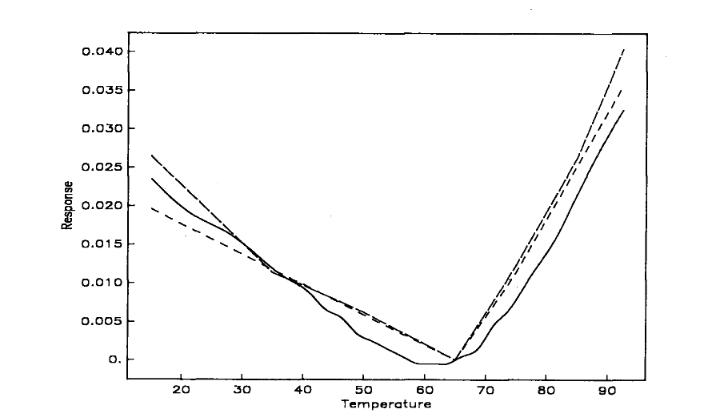
\includegraphics[scale=0.68]{graph1.png}
    \caption{Engle et al. pg. 316}
    \label{LitReviewImage1}
\end{figure}

The data shows a positive correlation between temperature and electricity usage. In our experiment, we measured these variables, along with other naturally occurring phenomena like wind and cloud cover. While Engle et al. focused on the percent change, our model focused on the actual correlation between these variables.


\section{Data-set Description and Analysis}\label{sec:3}
Our dataset contains two CSV files of four years of hourly data spanning from January 1, 2015 to December 31, 2018. It was generated from ENTSOE, a public portal that collects energy data for countries across the European Union, and the Open Weather API. The first CSV file contains 29 columns of energy related data such as price, total load, and energy generation from renewable and nonrenewable sources. This data had 35065 rows with all energies measured in megawatts, MW. The second file had 178397 rows of weather data such as temperature, wind speed, rain amount, and weather descriptors. The file had about five times the rows of the energy generation because contained data from five major Spanish cities: Valencia, Madrid, Barcelona, Bilbao, and Seville. This required an extra layer of data analysis and cleaning. Both datasets contained a "datetime" column, simplifying the process of combining them together.


Since the energy data represents all of Spain, we could not compare individual city data. Attempts to do this resulted in poor correlations between a single city and the energy dataset. We decided to take an average of the weather data for all cities to create a single dataset with the same number of rows as the energy data. Figures \ref{loadVsTemp1} and \ref{loadVsTemp2} below show a comparison between using a city's weather data and averaging the five cities’ weather data. Here, in Fig. \ref{loadVsTemp1}, where the data is averaged, we can see a clearer polynomial relationship between the total load and the temperature where the minimum of the total load occurs at 293K. Decreasing or increasing this temperature causes the total load to increase. 

Compare this to Fig. \ref{loadVsTemp2} where the density plot looks more like a random blob of points. Further, we see a limitation of the recording device in Fig. \ref{loadVsTemp2}. The tendency of points to fall on a vertical line is due to the recording device measuring to the precision of the decimal point. In other words, it's not very precise. This is hidden when the average is taken. We also tested a weighted average based on city population, but that resulted in worse correlations for standard regression models. This is because the weather is independent of population. However, that does not mean the weighted average performs worse when used in all the models, the neural network solution was able to perform better with the weighted average inputs.

\begin{figure}[H]
    \centering
    \begin{minipage}[t]{0.45\textwidth}
    \centering
    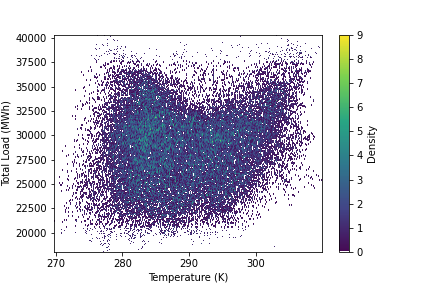
\includegraphics[width=.9\linewidth]{load_vs_temp.png}
    \captionof{figure}[TEM]{A density plot of total load and the average temperature of the five cities}
    \label{loadVsTemp1}
    \end{minipage}%
    \hfill
    \begin{minipage}[t]{0.45\textwidth}
    \centering
    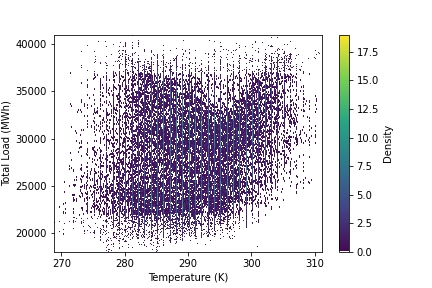
\includegraphics[width=.9\linewidth]{load_vs_temp_valencia.png}
    \captionof{figure}[TEM2]{A density plot of total load and the temperature in Valencia}
    \label{loadVsTemp2}
    \end{minipage}
\end{figure}%

\begin{figure}[ht]
    \centering
    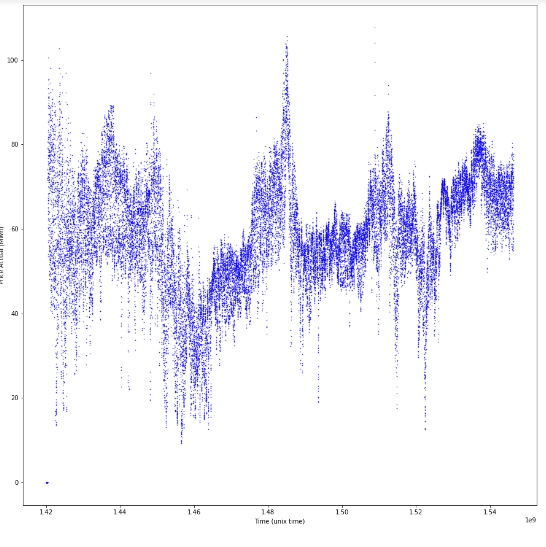
\includegraphics[scale=0.68]{graph2.png}
    \caption{A plot of price vs time in UNIX time}
    \label{priceVsTemp}
\end{figure}

We also found a correlation between time and price. From Fig. \ref{priceVsTemp}, we can see that price and time have a sinusoidal relationship due to the seasonality, and daily trends, in weather - in the summer, the weather is hotter and people power on their air conditioners, and at night, people use less electricity because they are asleep. 

To understand the importance of each feature a priori, we used a mutual information regression tool that relies on a non-parametric, entropy-based approach, to understand the significance of the relationship between the target (price) and each feature.  From Fig. \ref{featureImportances1} below, we see that our engineered features seem important for model performance.

\begin{figure}[ht]
    \centering
    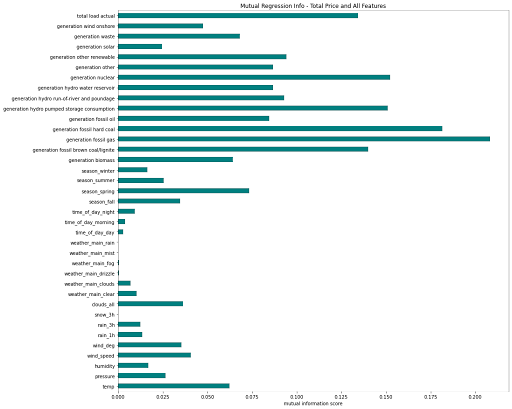
\includegraphics[scale=0.55]{feature_importances.png}
    \caption{A bar graph depicting how strongly a feature affects the price}
    \label{featureImportances1}
\end{figure}

\section{Proposed Methodology}\label{sec:4}
We propose a five step methodology.

\subsection{Determine Variables of Interest}
We picked total load and price to be our variables of interest due to their more practical applications - total load for businesses trying to determine a price and price for users trying to determine the optimal time to use electricity.

\subsection{Preprocessing}
All city data had duplicate rows save for the weather description - e.g. “few clouds” rather than “scattered clouds.” We removed the second row in all instances and assume this strategy will have minimal impact on our results. Columns that featured only, or were largely, NaNs or 0s, such as “generation hydro pumped storage aggregated” were removed. We leave the description of scaling to the experimental results section, as not all of our models require it (such as XGBoost, which is invariant to scale). 

As energy data was taken countrywide, the data obtained for the various cities were averaged together. 

\subsection{Feature Engineering}
As noted above, time of day and season were information-rich sources in the data. We decided to parse the time stamps to create a season feature - [spring, summer, winter, fall] - and a time of day feature - [day, morning, night]. For predicting total load, we used both aforementioned parsed time variables, temperature, humidity, pressure, wind speed, wind degree, rain, snow, and cloud coverage. 

As many energy generation variables were independent of weather, the primary goal was to predict the price given a total load. However, EDA showed other energy generations to have a larger impact on the predicted price. We therefore decided to develop two models with the goal of comparing the two: one that used only the total load and one that used the total load as well as the means at which the energy was produced. The only energy generation variables that were not included were those with only NaNs and 0s, or the “forecasted” values as actual values are a better measure for the price than the predicted ones.

\subsection{Model Training and Evaluation}
For our analysis we utilized several different machine learning methods and algorithms to find which one gave us a possible correlation between variables. Our main methodology was to find a regression model that matched and accurately predicted the outcome of later data. Our group ran many models such as ANNs, DNNs, XGBoost, and other various algorithms. Once each model is trained, we evaluate the model using MSE and R2 on both training and testing sets. During this process, we optimized for hyperparameters in XGBoost and NN using a grid search.

\subsection{Model Interpretability}
A critical component of any complex consumer-facing model is interpretability and explainability. To gain insight post-training in the XGBoost model, we use SHAPley values to understand which factors and features are the most important to predicting the price per MWh in euros and total load for our models.

\section{Experimental Results}\label{sec:5}

\subsection{Neural Network}

For the neural network, our goal was to produce a model that takes in a limited amount of variables to produce a longer range forecast on the total load. There currently exist many tools for accurately predicting future weather and we can use those predictions in our model. This is opposed to using variables that are only available at present, like weather observations or generation data. Using these limited variables, we can create a forecast for total load that is valid for any time the other variables are also valid.

After a grid search to tune hyperparameters, the neural network consisted of four layers, one five neuron input, two three-neuron hidden layers, and one single neuron output layer. For all layers except for the output, exponential linear unit (ELU) activation was used, and for the output layer, the hyperbolic tangent function (tanh) was used. The optimizer used was 'Adam' with a learning rate of 0.001. The model was trained for 500 epochs, with issues of non-convergence beyond this point with a lower learning rate and higher number of epochs. The five inputs into the neural network were time of day, temperature, humidity, cloud cover, and wind speed. This neural network was able to produce a training RMSE of 0.14 on min-max scaled data. The testing data had a similar RMSE of 0.14, and an R$^2$ value of 0.53, indicating that there was limited over-fitting, but generally low accuracy, but would still give us a ballpark estimate on the load.

\begin{figure}[H]
    \centering
    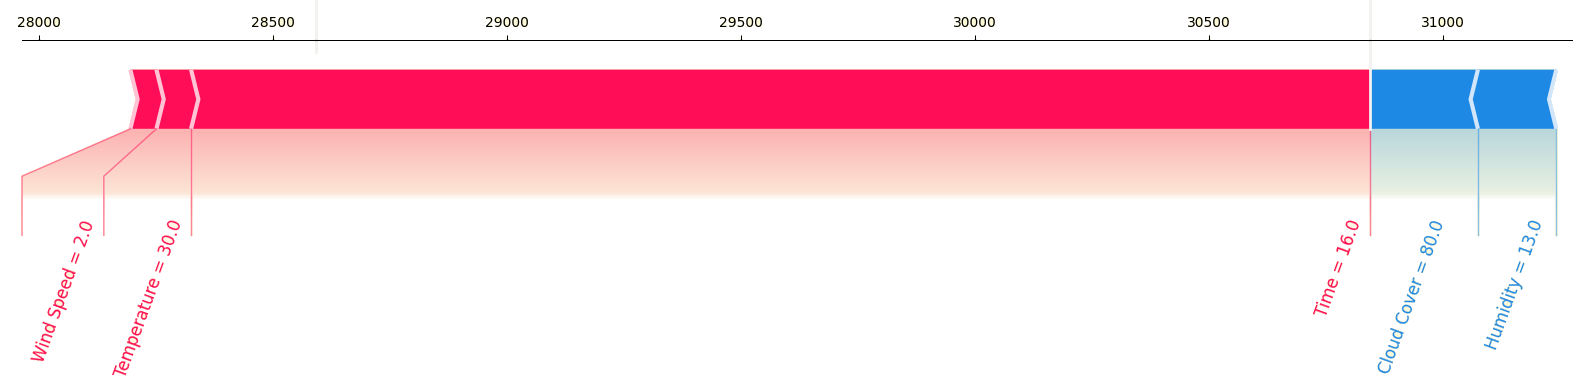
\includegraphics[scale=0.39]{shap_nn.png}
    \caption {The above figure is a SHAP force plot for a prediction using the neural network. Larger bars contributed more to the output.}
    \label{shap_nn}
\end{figure}

Based on the SHAP force plot in figure \ref{shap_nn}, we can see that the neural network assessed time of day as the most important variable in the prediction. This makes sense, as in the energy industry, usage during peak hours is more expensive and difficult to meet than usage during off-hours.

\subsection{Polynomial Regression}

As seen in \ref{featureImportances1}, the total load and other energy generation values affected the price more than the weather. Due to limitations of predicting methods of energy generation (many were not correlated with weather in any way), we wanted to predict the price given an estimated total load. As the dependent variable only depended on a singular independent variable in this case, we decided on a polynomial regression. 

In real life, while the price is dependent on the weather, in that people use more electricity when it’s cold or hot, this price is ultimately set based on the predicted total load - eg. prices are higher in the afternoons and lower at night due to higher energy usage in the afternoons. 

\begin{figure}[H]
    \centering
    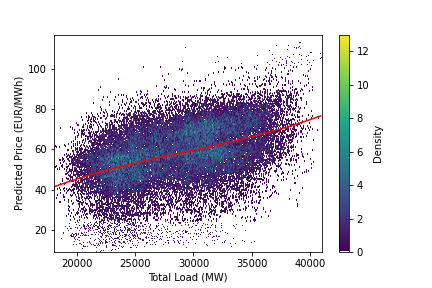
\includegraphics[scale=0.55]{polynomial_regression.png}
    \caption{A third-degree polynomial regression of the predicted price vs total load plotted on top of a density plot. This model had a training MSE of 163.18, a testing MSE of 162.87, a training RMSE of 12.77, a testing RMSE of 12.76, and an R2 of 0.19}
    \label{polyreg}
\end{figure}

Both the density plot and the polynomial regression in \ref{polyreg} above show a clear upward relationship between the two. This is because a greater total load means a higher demand for energy, which means the prices go up. However, as is also shown in Fig. x, our polynomial regression, with an R2 score of 0.19, was not very accurate. Our model was unable to capture the variance in the data.  

\subsection{XGBoost}

We selected XGBoost as it has high model capacity, prediction performance, and other performance benefits such as parallelism have given it widespread adoption in industrial applications. XGBoost is an ensemble model variant - ensembling occurs in a sequential fashion using gradient boosting. Each model in the ensemble is trained to correct the error of the previous model in the ensemble by updating its weights using the gradient of the loss function w.r.t. the previous’ models output (and thus, error). This allows for computational feasibility and heightened performance. Further, our data is tabular, a data form that XGBoost handles very well. Our results for predicting price were very good. The training R squared score was 0.991 while the testing R squared score was 0.917. Training mean squared error was 1.675 and training MSE was 16.127. XGBoost also lends itself nicely to a SHAP analysis, which we used to gain insights from our model.  SHAP values quantify the importance of a feature on a model’s prediction.

It is important to note that through grid search, our final XGBoost model had the following hyperparameters: learning rate of 0.06, max depth of 8, and 800 estimators.

\begin{figure}[H]
    \centering
    \begin{minipage}[t]{0.45\textwidth}
    \centering
    \hspace*{-2.5cm} 
    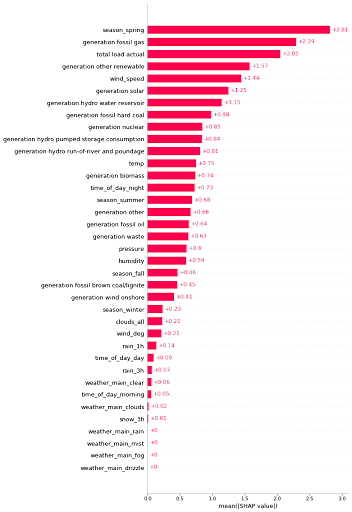
\includegraphics[width=1.2\linewidth]{shapbar.png}
    \captionof{figure}[TEM]{ SHAP bar graph}
    \label{shapbar}
    \end{minipage}%
    \hfill
    \begin{minipage}[t]{0.45\textwidth}
    \centering
    \hspace*{-2.5cm} 
    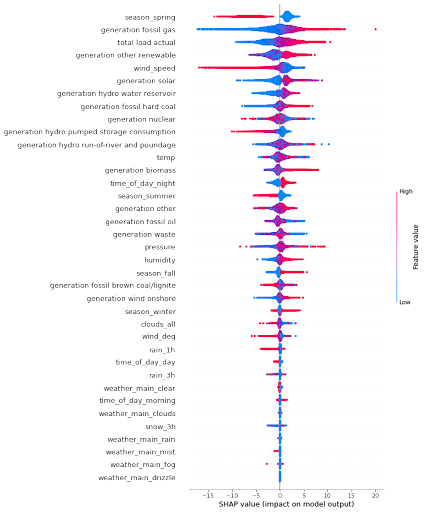
\includegraphics[width=1.4\linewidth]{shapbee.png}
    \captionof{figure}[TEM2]{SHAP beeswarm plot}
    \label{shapbee}
    \end{minipage}
\end{figure}



From \ref{shapbar}, we learned that the season being spring or not had the most impact on the price prediction. From \ref{shapbee}, we can see that the spring season decreases the price, and vice versa. From \ref{shapbar}, we know that the generation of fossil gas is the second most important, and \ref{shapbee} shows that high fossil fuel generation levels increase the price.  A similar analysis can be conducted on the other variables.

\section{Conclusion and Discussion}\label{sec:6}
Using energy and weather data, we were able to predict total load and price using a variety of models and feature choices. After these experiments, we learned that energy price prediction involves multiple factors that all play different, but important roles. Despite total load having a strong correlation with price actual, we saw that a simple polynomial regression did not capture the complexity of the data sufficiently.

The neural network had decent performance in regards to predicting total load, under the consideration that it does not take in many variables. All the variables that the neural network takes as inputs are also available as forecasts, meaning that although the accuracy of the total load forecast may not be the strongest, we can make reasonable forecasts for a large timeframe, including days in the future.

The total load forecast from the neural network can be used to predict price using our polynomial regression model. A problem with the model was that it was unable to capture the variance in the total load data. This high variance could be due to a variety of factors, including individual electricity consumption vs business energy consumption, or not taking into account the day of the week, or holidays. 

Though our XGBoost model had the highest R2 among all three models, this required the inclusion of energy production sources. But predicting generation from each source is more difficult than predicting the weather. Thus, the ideal goal would be to predict the price using only the total load or weather variables. 

Through our discussions with industry experts and also our literature review, we found that the weather is typically a very good indicator of total energy consumption, which our model did not pick up on. This may be due to trying to model the energy consumption of an entire country given only five cities. This, however, may not be the best representation of the country. For starters, these five cities don’t cover the more arid desert land of Spain. Another thing is that by averaging the city’s weather data, we decrease the variance in our used dataset - eg. a colder than a normal day in Valencia would be damped out by the warmer weathers in the other four cities. An alternative to averaging the weather data would be to create 5 features for each weather variable, one associated with each city. Or, given city data, it would be best to estimate city energy consumption rather than country energy consumption. 

\section{GitHub Repository with Code}

\url{https://github.com/LunarZephyr/ECS171_Project}



\newpage
\begin{thebibliography}{9} 
    \bibliographystyle{apalike}
	\bibitem{XGBoost} Chen, T., \& Guestrin, C. (2016). XGBoost. Proceedings of the 22nd ACM SIGKDD International Conference on Knowledge Discovery and Data Mining. https://doi.org/10.1145/2939672.2939785 
	
	\bibitem{unknown} Jhana, Nicholas. (2019) Kaggle https://www.kaggle.com/datasets/nicholasjhana/energy-consumption-generation-prices-and-weather
	
	\bibitem{A Unified Approach to Interpreting Model Predictions} Lundberg, S., Lee, S. (2017) A Unified Approach to Interpreting Model Predictions. Advances in Neural Information Processing Systems 30 (NIPS 2017). https://doi.org/10.48550/arXiv.1705.07874
	
	\bibitem{Semiparametric Estimates of the Relation Between Weather and Electricity Sales} Engle, R., Granger, C.W., et al. (1986) Semiparametric Estimates of the Relation Between Weather and Electricity Sales Journal of the American Statistical Association Vol. 81, No. 394. tandfonline.com/doi/pdf/10.1080/01621459.1986.10478274
	
	\bibitem{Large-Scale Machine Learning on Heterogeneous Distributed Systems} Abadi, M. et al. (2015) Large-Scale Machine Learning on Heterogeneous Distributed Systems (Tensorflow).
	https://doi.org/10.48550/arXiv.1603.04467
	
	\bibitem{Scikit-learn: Machine Learning in Python} Pedregosa, F. et al. Scikit-learn: Machine Learning in Python. (2011) Journal of Machine Learning Research 12 2825-2830.
	https://dl.acm.org/doi/10.5555/1953048.2078195
	
	\bibitem{unknown} ENTSOE Energy API.  https://github.com/EnergieID/entsoe-py.
	
	
	
	
	
\end{thebibliography}

\newpage
\section{Customer Discovery Report}\label{sec:7}
\subsection*{Customer Discovery Report}
The study of meteorology can be extrapolated to many different companies whose industries rely on a particular weather in one way or another. Our report primarily focuses on the five biggest cities in Spain, however, most of the interviews we conducted were done primarily in California. The variability in climate is not 1-to-1 but we can use the information that we have collected to show the importance of weather on a greater scale. Our interviews were conducted with various professors and engineers that are currently working in the field and are directly or indirectly working with machine learning methods. 

\subsubsection*{Interview with Professor Ellis of UC Davis}
Our first customer that we reached out to for comment and review on our analysis of the weather trends in Spain was Professor Ellis. He is a chemical engineering professor at UC Davis who uses machine learning algorithms to predict energy usage in buildings. His primary goal is to minimize energy use by improving process control in the energy systems. The first question that we asked all our interviewees was, “what are your critiques of our report and how do you think that it is applicable to a real life situation”. He responds, “They’re predicting energy usage in buildings, the solutions are accurate, and weather is a good indicator for demand. I could definitely see this as being a model that could be used with a lot of work”. According to Professor Ellis, something that we did correctly was breaking up the country into climate zones, however we should have taken into consideration the variety of climate zones in each of these areas and that the mean may not yield accurate results. A better way that we should have approached the problem is to determine the differences in climates of the cities, get data from mountainous regions, and sample a wider variety of cities to reduce other confounding variables. With all of these taken into account, we could have a greater understanding of the data as a whole and with more complicated modeling methods.


\subsubsection*{Interview with Sanjay Priyadarshi of Bloomreach Inc}
Sanjay is a customer success manager at Bloomreach that specializes in delivering products to customers by streamlining the process of SaaS to customers and using data to provide strong evidence for market movements and business solutions. I asked him about how our project relates to a business standpoint and he gave us some valuable insights to our report and where it plays a role in industry. Many industries that are related to sports or entertainment have a lot of information about the weather and the effects on players and viewers. One thing that was brought up was how weather is an important factor in games like cricket, baseball, and football. Most of these sports take place in open stadiums and there are huge masses that come to attend these events. The seasons for these sports are strategically chosen to be played during a certain season because of the positive weathers associated with that season. One example of this is baseball that is often played in the summer months and relies on the good weather and heat for large attendance and ease of play for the players purely based on the fact that baseball is hard to play in the rain and snow. In this way, machine learning is a prime example of how we can figure out using the probability of weather, the chances and the general trends in weather to find the time period in which it will rain, snow, or have unpredictable weather. Although from what we discussed, Sanjay could not really say that the weather project was a big part of the role and business that he played, he acknowledged that machine learning in his team has a primary purpose: making sense of unorganized data on a large scale by making meaningful predictions out of it.

\subsection*{Interview with Shivajee Samdarshi of Venafi}
In the Bay Area, there are several different technologies that are relevant to forecasting that require machine learning techniques and methods to make predictions that are consistent and valuable. Shivajee Samdarshi, currently the Vice President of Venafi, formerly an engineer at TIBCO, explained the importance of machine learning and how our product would benefit customers that use his company's services. Venafi is a cybersecurity company that provides services like certificates to customers and TIBCO provides business data to its customers for use and querying. When talking to Shivajee about our project we discovered that there were many technologies that TIBCO provided that showed the sheer power of machine learning and the applications to business. Of the many products that TIBCO provides, one that was interesting and we went into detail of TIBCO MDM and TIBCO BusinessEvents which are both data virtualization and translation softwares. Previously in Sanjay’s interview, we talked about how data can be used by businesses and with Shivajee’s interview we talked about how TIBCO can use the data and interpret it and provide it to the customer. Going back to the example of sports teams like the MLB that requires weather information to make good decisions on when and where games could be played, TIBCO’s computation services and machine learning products could help provide insightful and predictive analytics on where and when these games can be played. Shivajee also gave useful insight into how important weather forecasting is for normal ordinary people. Hundreds of millions of users around the world use services like Google to check the upcoming weather every morning and a reliable source of information is needed, which is something our machine learning model, if extrapolated to a higher extent can provide.

\subsection*{Interview with Amir Javanbakht of CAL ISO}
Specific to energy prediction, there is a demand for statistical analysis of energy usage. According to Amir, an analyst who works to predict and report energy usage for the state of California, the most important thing with predicting usage is understanding human behavior. "When you have data for a specific area, before you attempt to perform any regressions or develop models, you have to make an attempt at understanding it." By this, he meant that there are many ways to frame the data. Energy usage can be affected by things like day of the week, whether it is a holiday, time of day, temperature, wind speed. Gaining an understanding of how these variables might affect the output variable, whether it is an increase or decrease, and how significant is the trend, allows you to develop better statistical models. To create these models, Amir stated that he uses software like SAS and Itron specifically allows for easy interfacing between real energy data and creating statistical models, even machine learning models. However, he did say that the industry is moving towards open source solutions, and many of his colleagues are switching to python and R. For our machine learning solution specifically, the way to get better correlations and performance would be to break up our data into smaller variables which have an explicit relationship to our dependent variable. Overall, machine learning is very promising in the field of energy prediction, and Amir is excited to see where it might lead the industry.

\subsection*{Interview with Weather Forecaster Jim Tang}
Jim Tang is a weather forecaster that specializes in the forecast of severe weather in the plains. The tools he uses for forecasting are mainly deterministic models, or models that use the laws of physics in order to generate a solution for the state of the atmosphere in the future. "There are many different models that all have slightly different takes on what might end up occurring in the future. It is our job as forecasters to evaluate which models have been performing well, and weight our official forecast on the models that have been performing well, as well as an objective, common sense, analysis on how weather systems usually behave." This is an area where Jim believes that machine learning can help. Having a machine learning model assist in analysis of different deterministic models would be useful in bringing consistency in forecasts, and help prevent bias in forecasters. There are already small scale proof of concept ideas that execute this function, most of them powered by neural networks. One of them is called Nadocast, which a machine learning solution to try to predict areas where tornadoes might be more likely. The output of this model is similar to forecasts produced by official forecast agencies, and he said that it is a tool that he likes to use when determining where severe weather might occur. Jim closed by saying that there are countless other opportunities to use machine learning to assist in the human side of forecasting.

\end{document}